\documentclass{article}
% Official NeurIPS 2026 style (media.neurips.cc, Formatting_Instructions_For_NeurIPS_2026.zip).
% [preprint] shows the author and prints "Preprint." in the footer: this is a course report,
% not a NeurIPS submission or publication.
\usepackage[preprint,nonatbib]{neurips_2026}
\usepackage[utf8]{inputenc}
\usepackage[T1]{fontenc}
\usepackage{hyperref}
\usepackage{url}
\usepackage{booktabs}
\usepackage{amsmath,amssymb}
\usepackage{microtype}
\usepackage{graphicx}
\usepackage{xcolor}
\usepackage{enumitem}
\setlist{nosep,leftmargin=1.2em}

\title{How Much Expert Data Does Offline RL Need?\\
Behavior Cloning vs.\ Implicit Q-Learning on Mixed-Quality Hopper Datasets}

\author{Rahul Vishnuvardhana\\
Khoury College of Computer Sciences, Northeastern University\\
CS 5180 Reinforcement Learning, final project report}

\begin{document}
\maketitle

\begin{abstract}
We mix expert and low-quality Hopper data at five expert fractions $p\in\{0,0.05,0.2,0.5,1\}$ and train behavior cloning (BC) and Implicit Q-Learning (IQL) on each, with 5 seeds, 300k gradient steps, one commit and one CPU type (70 runs). Three hypotheses and their tests were pre-registered before any grid result existed. BC's score rises with $p$ (supported, +23.2 points from $p=0$ to $p=1$), but it stays at about 82 from $p=0$ to $p=0.5$ and rises only between $p=0.5$ and $p=1$ (nothing in between was run). IQL does not reach near-expert performance at a lower $p$ than BC (not supported): both cross 90 only at $p=1$, where IQL trails BC by 5.7 points. With little expert data IQL collapses: at $p=0.05$ it scores 6.7 and falls in 98\% of episodes, against BC's 82.2 with no falls. Whether a higher expectile $\tau$ helps more at $p=0.05$ than at $p=0.5$ is inconclusive; the observed effect points the other way.
\end{abstract}

\section{Problem and setup}
Offline RL learns a policy from a fixed dataset without interacting with the environment [9]; improving on the data requires values for actions the data rarely contains [10]. Real logs mix good and poor behavior, so we make the \emph{fraction of expert data} the independent variable and ask how quickly imitation (BC) and in-sample value learning (IQL [1]) reach expert performance as it grows.

\textbf{Related work.} On D4RL Hopper, BC barely changes from \texttt{medium} to \texttt{medium-expert} data while IQL improves strongly [1,3]; our low-quality data is much stronger than D4RL's medium data (BC scores 82 on it) and our mixtures hold fewer expert transitions, so we read our results as a different regime rather than a contradiction. Hong et al.\ [11] mix 1, 5, 10 or 50\% expert or medium data with random data and find that uniformly sampled offline RL, IQL included, fails to exploit scarce high-return data, which reweighting trajectories by return largely mitigates; our IQL does something worse than failing to improve, since adding expert data drops it below its own score on the low-quality data alone. Kumar et al.\ [12] characterize when offline RL should beat BC (for example, when only a few states are critical), Park et al.\ [13] find that the policy extraction step often limits performance more than value learning, with advantage-weighted regression extracting worse policies than DDPG+BC, and Schweighofer et al.\ [14] find BC competitive with offline RL when trajectory quality is high, as it is even for our weaker dataset.

\textbf{Environment and data.} Gymnasium Hopper-v5 on MuJoCo [6,7] (11-D state, 3-D action in $[-1,1]^3$). Two Minari datasets [5]: \texttt{expert-v0} (999,164 steps) and \texttt{simple-v0} (999,206 steps; a weaker SAC policy that hops slowly). Each mixture has 900k transitions, of which a fraction $p$ comes from expert episodes, sampled as whole episodes; mixture seed $s$ fixes the file, shared by every method at that $p$. Simple episodes are shorter (about 510 vs.\ 920 steps; they fall more often), so expert episodes are a smaller share of \emph{episode starts} than $p$: about 50 of 1,700 (3\%) at $p=0.05$, 12\% at $0.2$ and 36\% at $0.5$ (mixture seeds 0 to 2). A fall is a termination; the 1,000-step time limit is not.

\textbf{Methods.} Both use the same Gaussian policy (256-256 MLP, state-independent std) and the same buffer, state normalization, evaluation and budget. BC maximizes $\log\pi(a\mid s)$. IQL fits $V$ by expectile regression on $Q$, $Q$ by TD toward $V(s')$, and the policy by advantage-weighted regression [4] with $\beta=3$; $\tau=0.7$ in the main grid, $\tau\in\{0.5,0.9\}$ in the ablation; rewards are scaled by $1000/(\max_\text{ret}-\min_\text{ret})$ over the mixture's complete episodes. BC is IQL's policy loss with $\beta=0$, so the two differ in one design choice: whether imitation is weighted by a learned advantage. IQL was checked against CORL's implementation [8] before the grid (step-for-step equality in tests; real-data runs at $p\in\{0.2,1\}$; see Limitations). All hyperparameters except the 300k-step budget (the IQL paper uses 1M) follow the IQL paper's MuJoCo setting; they are listed in Appendix~\ref{app:hparams}.

\textbf{Score.} $100\,(R-r_\text{random})/(r_\text{expert}-r_\text{random})$, with $r_\text{random}=17.03$ and $r_\text{expert}=3857.80$ the expert dataset's mean return. A run's final score is the mean of its last 5 evaluations (280k to 300k steps), each 50 episodes on fixed evaluation seeds; its fall rate is the fraction of those 250 episodes that end in a fall.

\textbf{Pre-registration.} Hypotheses, tests and verdict rules were fixed on 2026-11-21, before any grid result. Development runs on other seeds, which enter no verdict, had already shown IQL far below BC at $p=0.2$ and behind it at $p=1$; the pre-registration lists them, so H2 was fixed knowing it might fail. Each test is the exact one-sided paired sign-flip test on the 5 per-seed values (all $2^5=32$ sign patterns), level 0.05; we write $P$ for these $p$-values to keep $p$ for the expert fraction. With 5 seeds a test rejects only when all 5 seeds agree ($P=1/32=0.031$), so power is low and ``inconclusive'' is not evidence of no effect. Intervals (95\% t, and percentile bootstrap over seeds, 10,000 resamples) are indicative only: 5 seeds allow only 126 distinct bootstrap resamples. \textbf{There is no correction for multiple comparisons across H1 to H3}: each verdict's false-positive rate is $1/32$, so the chance of at least one false positive among the three is at most $3/32\approx0.094$ if all three null hypotheses hold.

\textbf{Compute.} One commit (\texttt{ea11e14}), CPU only (Intel Xeon Platinum 8276, 4 cores per run) on Northeastern's Explorer cluster; 70 runs in 3.1 hours of wall clock, 195 CPU-hours, no failures or reruns.

\section{Results}
\begin{figure}[t]
  \centering
  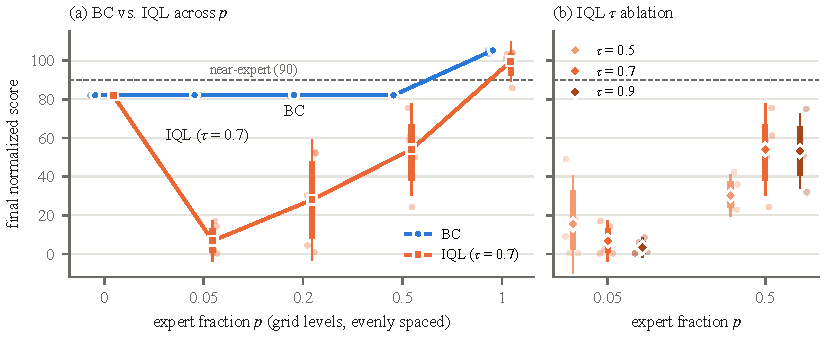
\includegraphics[width=\linewidth]{../figures/score_vs_p.pdf}
  \caption{Final normalized score (5 seeds). Dots: individual seeds; markers: seed mean; thin whisker: 95\% t-interval; thick bar: 95\% bootstrap interval; dashed: near-expert threshold (90). (a) BC and IQL ($\tau=0.7$) at every $p$; grid levels are evenly spaced although uneven in $p$. (b) IQL's $\tau$ ablation at $p=0.05$ and $0.5$, with $\tau=0.7$ from the main grid.}
  \label{fig:main}
\end{figure}

\begin{table}[t]
  \caption{Pre-registered verdicts. $\bar d$: mean of the 5 per-seed differences; $P$: one-sided exact $p$-value.}
  \label{tab:verdicts}
  \centering\footnotesize
  \begin{tabular}{@{}l@{\hspace{4pt}}p{0.30\linewidth}r@{\hspace{5pt}}l@{\hspace{5pt}}r@{\hspace{5pt}}l@{}}
    \toprule
    & Test (one-sided, greater) & $\bar d$ & Per seed & $P$ & Verdict \\
    \midrule
    H1 & BC($p{=}1$) $-$ BC($p{=}0$) & $+23.2$ & 23.2, 21.3, 24.1, 23.0, 24.4 & 0.031 & \textbf{Supported} \\
    H2 & IQL $-$ BC at IQL's crossing $p$ (1; BC's is also 1) & $-5.7$ & $-4.4, -0.1, -2.2, -19.4, -2.3$ & 1.000 & \textbf{Not supported} \\
    H3 & $[\tau_{.9}{-}\tau_{.5}]_{p=.05} - [\tau_{.9}{-}\tau_{.5}]_{p=.5}$ & $-35.0$ & $-61.6, -22.6, -57.2, -38.2, +4.6$ & 0.969 & \textbf{Inconclusive} \\
    \bottomrule
  \end{tabular}
\end{table}

\textbf{H1, BC's score rises with $p$: supported.} BC($p{=}1$) exceeds BC($p{=}0$) on all 5 seeds ($+23.2$; t-interval $[21.7, 24.7]$; pre-registered $P=0.031$, the primary result). \emph{Secondary, not pre-registered:} the 5 values at $p=1$ all exceed the 5 at $p=0$, so an exact one-sided unpaired rank (Mann-Whitney) test gives $P=1/252\approx0.004$. The rise is a step, not a slope (Fig.~\ref{fig:main}a): BC scores 82.2, 82.2, 82.2 and 82.1 at $p=0$ to $0.5$ and 105.4 at $p=1$, and no adjacent drop exceeds 5 points, so BC is monotone as far as 5 seeds show (mean per-seed Spearman correlation with $p$: 0.46). The pre-registered dip check flags $p=0.05$ and $0.5$, but by under 0.1 point (adjacent-drop $P\geq0.156$): no averaging failure of practical size appears. Even with half the transitions from expert episodes, BC matches what it learns from the low-quality data alone. BC scores above both datasets' own means (82 vs.\ 42.7, and 105.4 vs.\ 100) because its deterministic mean action rarely falls, while the data falls in 66\% (simple) and 28\% (expert) of episodes; BC's episodes that do not fall return about what the data's do (development runs at 100k steps: 3,169 vs.\ 3,179 simple, 4,104 vs.\ 4,157 expert). This is why plain imitation is hard to beat here, and one reason our results differ from D4RL's.

\textbf{H2, IQL reaches near-expert ($\geq 90$) at a much lower $p$ than BC: not supported.} The smallest $p$ from which a method's mean stays at or above 90 is $p=1$ for both, so IQL does not cross lower. At $p=1$ IQL scores 99.7 and trails BC (105.4) on all 5 seeds. Below $p=1$ IQL is far worse than BC: by $-75.4$, $-54.3$ and $-28.0$ points at $p=0.05$, $0.2$ and $0.5$, with BC ahead on all 5 seeds at each (one-sided $P=0.031$; at $p=1$ also 0.031). \emph{These ``BC leads'' tests (IQL minus BC, opposite to H2) are exploratory: the comparisons were pre-registered only as descriptive, and the tests are uncorrected.} At $p=0$ the two are within 0.2 points (descriptive).

\textbf{H3, higher $\tau$ helps more at $p=0.05$ than at $p=0.5$: inconclusive, observed in the opposite direction.} The contrast is negative on 4 of 5 seeds ($-35.0$). The simple effects: raising $\tau$ from 0.5 to 0.9 changes IQL by $-12.1$ at $p=0.05$ (15.3 to 3.2) and by $+22.9$ at $p=0.5$ (30.2 to 53.1). The pre-registered reverse-direction test, used only to label a reversal, gives $P=0.0625$, so H3 is not labelled reversed: seed 4 alone prevents it. H3 carries little information in this design: IQL is near the floor at $p=0.05$ for every $\tau$, which compresses the contrast, and changing $\tau$ also changes the scale of the advantages and hence of IQL's policy weights, so the ablation does not isolate the expectile.

\textbf{IQL's collapse comes with falls.} Pre-registered flags mark a run \emph{high-fall} if it falls in at least half of its final episodes and \emph{collapsed} if it scores below 10; flagged runs stay in every statistic. Every IQL run at $p=0.05$ is high-fall (fall rate 0.88 to 1.00 per cell) and 11 of 15 collapsed; at $p=0.2$ and $0.5$, 4 and 3 of 5 $\tau=0.7$ runs are high-fall. BC never falls below $p=1$, and at $p=1$ its fall rate is 0.03 on average (one seed 0.14). With scarce expert data, IQL's policies fall; at $p=0$ (simple data only) it is nearly stable (fall rate 0.02). A side-by-side video of each $p=0.05$ cell's median-scoring run (final policies, evaluation seed 10000, the logged episode replayed exactly) is in the repository: BC hops for all 1,000 steps, IQL falls after 27.

\textbf{Post hoc diagnostic (not pre-registered; a candidate mechanism, not a finding).} After the grid, a review probed the saved final policies and critics of a few runs without retraining, using their own mixtures and evaluation rollouts of 10 to 20 episodes (supplementary review record, submitted with this report). Expert and simple episodes start from the same initial-state distribution and diverge within about 3 steps. \emph{First-action lock-in, clearest at $p=0.05$:} in seed 1, IQL's critic rates the 49 expert first steps far above the 1,681 simple ones (advantage about 10 vs.\ $-0.8$), so 48 of the 49 expert weights $e^{\beta A}$ hit the clip of 100 and IQL's first action copies the expert's, while BC's copies the simple data's. With only 49 expert episodes IQL then falls, and so does BC when handed an expert first action (33 and 35 points, two runs). Replacing only IQL's first action with BC's raised IQL from about 0.4 to between 71 and 83 in three runs ($p=0.05$ seeds 1 and 3, $p=0.2$ seed 3) and improved all nine runs checked ($p=0.05$ to $0.5$), though in 4 of them falls remained (20 to 65\% of episodes). \emph{Weaker gait-following, from $p=0.2$ up:} given the same expert first action, BC continued the expert gait better than IQL by 36 and 40 points in the two runs checked at $p=0.2$ and $0.5$, and on expert transitions IQL's squared action error exceeds BC's by 11 to 17\% in three runs at $p=0.2$ and $0.5$ but by only 3.5\% at $p=1$. These checks cover few runs and were chosen after seeing the results; they explain where IQL loses, not how to make it win, and no variant of IQL tested here beats BC.

\begin{figure}[t]
  \centering
  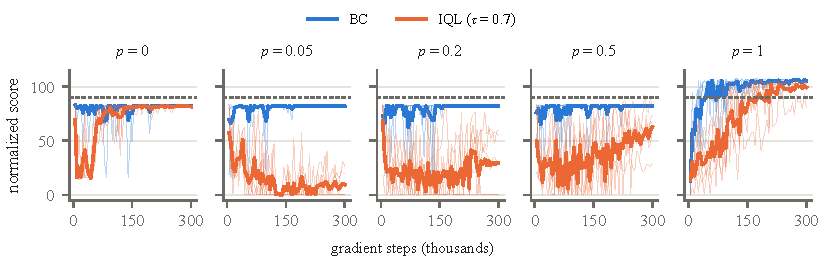
\includegraphics[width=\linewidth]{../figures/learning_curves.pdf}
  \caption{Learning curves (descriptive): score on the 10 evaluation seeds shared by every evaluation, every 5k steps; thin lines are seeds, thick lines their mean; dashed: 90.}
  \label{fig:curves}
\end{figure}

\textbf{Learning curves (Fig.~\ref{fig:curves}, descriptive).} IQL's failure at low $p$ develops during training: at $p=0.05$ and $0.2$ its seed mean is highest at the first evaluation (57.4 and 68.4 at 5k steps) and falls to 9.5 and 29.4 by 300k (curve values on 10 seeds; Table~\ref{tab:scores} uses the last 5 evaluations, 250 episodes), while BC is near 82 by 50k steps and stays there apart from brief single-seed dips. At $p=0$ IQL drops to about 16 within 10k steps and recovers to 81.7 by 300k; at $p=0.5$ its late evaluations still swing by several points between checkpoints (late-training fragility, Limitations); at $p=1$ it rises more slowly than BC (39.2 vs.\ 103.5 at 50k).

\textbf{Takeaway.} Two separate observations, on this dataset pair with IQL's default MuJoCo settings at 300k steps. (i) \emph{IQL collapses on mixtures:} at each tested $p$ strictly between 0 and 1 (0.05, 0.2, 0.5) it scores far below BC and below its own score on the low-quality data alone (82.0 at $p=0$), and most of its episodes end in falls. Training makes this worse, not just unhelpful: at $p=0.05$ and $0.2$ IQL is at its best at the first evaluation (57.4 and 68.4 at 5k steps) and declines to 9.5 and 29.4 by 300k. (ii) \emph{IQL also trails BC slightly on expert-only data:} by 5.7 points at $p=1$ (median per-seed gap 2.3; one seed's gap is 19.4). Separately, BC gains nothing from expert data until $p=1$ (no $p$ between 0.5 and 1 was run).

\begin{table}[t]
  \caption{Final scores per cell (5 seeds): mean, median, 95\% t-interval, mean fall rate, and the number of high-fall (HF) and collapsed (C) runs. Plateau: seed mean of the last 5 minus the previous 5 evaluations on shared seeds (pre-registered; values above 2 we read as late-training fragility, not continued learning; see Limitations).}
  \label{tab:scores}
  \centering\small
  \begin{tabular}{@{}llrrrrrrr@{}}
    \toprule
    Method & $p$ & Mean & Median & t-interval & Fall & HF & C & Plateau \\
    \midrule
    BC & 0 & 82.2 & 82.2 & [82.0, 82.3] & 0.00 & 0 & 0 & 0.0 \\
    BC & 0.05 & 82.2 & 82.2 & [82.0, 82.4] & 0.00 & 0 & 0 & 0.0 \\
    BC & 0.2 & 82.2 & 82.2 & [82.1, 82.3] & 0.00 & 0 & 0 & 0.0 \\
    BC & 0.5 & 82.1 & 82.2 & [81.8, 82.4] & 0.00 & 0 & 0 & $-0.1$ \\
    BC & 1 & 105.4 & 105.5 & [104.0, 106.8] & 0.03 & 0 & 0 & 0.2 \\
    \midrule
    IQL $\tau{=}0.7$ & 0 & 82.0 & 82.0 & [81.7, 82.4] & 0.02 & 0 & 0 & 0.1 \\
    IQL $\tau{=}0.7$ & 0.05 & 6.7 & 2.1 & [$-3.3$, 16.8] & 0.98 & 5 & 3 & $-0.5$ \\
    IQL $\tau{=}0.7$ & 0.2 & 28.0 & 30.1 & [$-2.9$, 58.9] & 0.77 & 4 & 2 & $-1.4$ \\
    IQL $\tau{=}0.7$ & 0.5 & 54.1 & 59.0 & [30.5, 77.6] & 0.61 & 3 & 0 & 5.4 \\
    IQL $\tau{=}0.7$ & 1 & 99.7 & 103.5 & [89.9, 109.5] & 0.10 & 0 & 0 & 1.5 \\
    \midrule
    IQL $\tau{=}0.5$ & 0.05 & 15.3 & 8.9 & [$-9.8$, 40.4] & 0.88 & 5 & 3 & 6.7 \\
    IQL $\tau{=}0.5$ & 0.5 & 30.2 & 26.4 & [19.6, 40.8] & 0.90 & 5 & 0 & $-4.8$ \\
    IQL $\tau{=}0.9$ & 0.05 & 3.2 & 0.9 & [$-1.6$, 7.9] & 1.00 & 5 & 5 & 0.8 \\
    IQL $\tau{=}0.9$ & 0.5 & 53.1 & 53.2 & [34.1, 72.2] & 0.73 & 4 & 0 & $-1.6$ \\
    \bottomrule
  \end{tabular}
\end{table}

\section{Limitations}
\begin{itemize}
  \item \textbf{Five seeds, low power.} Each test can only reach $P=0.031$ with all five seeds agreeing (changes from the proposal: Appendix~\ref{app:changes}); ``inconclusive'' (H3) is not evidence of no effect. No correction across H1 to H3; the pre-registered reverse-direction tests (H1, H3) only label a reversal; the per-$p$ ``BC leads'' tests are exploratory and uncorrected.
  \item \textbf{One environment, one dataset pair, Minari not D4RL [3].} All results apply to these two datasets only: seeds vary initialization and which episodes are sampled, not the source datasets. The scores are not comparable with D4RL's published numbers, and the simple data here is far better than random (BC on it scores 82), which may make imitation unusually strong. Filtered BC (imitating only high-return episodes) and a second offline RL method were not run.
  \item \textbf{IQL validation.} Against BC at $p=1$ on development seeds 100 and 101, our IQL missed the pre-fixed V1 margin (85.3 vs.\ 105.1); a follow-up on seeds 102 to 104 found it below CORL's IQL by more than 5 points on 1 of 3 seeds, recorded as seed variance. The CORL comparison \textbf{shared our preprocessing} (state normalization and reward scaling), so it validates the update code, not CORL's full pipeline; CORL's own state normalization is the same formula, and its reward scale differs from ours by 0 to 9\% on the mixtures we measured.
  \item \textbf{Fixed hyperparameters.} $\beta=3$ and the published MuJoCo settings were not tuned for mixtures; IQL's collapse at low $p$ may depend on them. The per-mixture reward scale is 0.25 to 0.27 for every $p>0$ but 1.46 times larger at $p=0$, so IQL's effective inverse temperature there is about 4.4 instead of 3 (sharper weighting). The policy is a single Gaussian, which cannot represent two gaits at once.
  \item \textbf{Late-training fragility, 300k steps only.} The pre-registered plateau statistic exceeds 2 points in two cells (IQL $\tau=0.7$ at $p=0.5$, +5.4; $\tau=0.5$ at $p=0.05$, +6.7), but over the final 20k steps the cosine schedule holds the actor's learning rate below 2\% of its initial value, and IQL's per-seed scores still change by several points between consecutive evaluations while BC's barely move. We read this as fragility of IQL's late policies, not continued learning; whether longer training changes the results is untested.
\end{itemize}

\section{Future work}
Two follow-ups would test the post hoc mechanism, each under its own dated pre-registration and on the reserved evaluation seeds 10050 to 10099. \emph{Stage 0 (evaluation only, existing checkpoints):} let IQL's critic choose only the first action and BC act afterwards, with controls that give BC an expert-mean or filtered-BC first action instead; it is a diagnostic and cannot count as an IQL win. \emph{Stage 1 (training, fresh mixture seeds 5 to 9):} keep IQL's critic but change policy extraction (DDPG+BC [13], or IQL with its weights floored at 1 or clipped at 2), alongside filtered BC and return-weighted BC baselines [11]; success would be a cell mean at least 5 points above plain BC with every paired difference positive, at both $p=0.2$ and $0.5$, with fall rates reported.

\section*{References}
{\small
\begin{enumerate}[label={[\arabic*]},leftmargin=2em]
\item I. Kostrikov, A. Nair, S. Levine. Offline Reinforcement Learning with Implicit Q-Learning. ICLR, 2022.
\item A. Kumar, A. Zhou, G. Tucker, S. Levine. Conservative Q-Learning for Offline Reinforcement Learning. NeurIPS, 2020.
\item J. Fu, A. Kumar, O. Nachum, G. Tucker, S. Levine. D4RL: Datasets for Deep Data-Driven Reinforcement Learning. arXiv:2004.07219, 2020.
\item X. B. Peng, A. Kumar, G. Zhang, S. Levine. Advantage-Weighted Regression. arXiv:1910.00177, 2019.
\item O. G. Younis et al. Minari. Farama Foundation, 2024. \url{https://minari.farama.org}.
\item E. Todorov, T. Erez, Y. Tassa. MuJoCo: A Physics Engine for Model-Based Control. IROS, 2012.
\item M. Towers et al. Gymnasium: A Standard Interface for Reinforcement Learning Environments. arXiv:2407.17032, 2024.
\item D. Tarasov, A. Nikulin, D. Akimov, V. Kurenkov, S. Kolesnikov. CORL: Research-Oriented Deep Offline Reinforcement Learning Library. NeurIPS Datasets and Benchmarks, 2023.
\item R. S. Sutton, A. G. Barto. Reinforcement Learning: An Introduction, 2nd ed. MIT Press, 2018.
\item S. Levine, A. Kumar, G. Tucker, J. Fu. Offline Reinforcement Learning: Tutorial, Review, and Perspectives on Open Problems. arXiv:2005.01643, 2020.
\item Z.-W. Hong, P. Agrawal, R. Tachet des Combes, R. Laroche. Harnessing Mixed Offline Reinforcement Learning Datasets via Trajectory Weighting. ICLR, 2023.
\item A. Kumar, J. Hong, A. Singh, S. Levine. When Should We Prefer Offline Reinforcement Learning Over Behavioral Cloning? ICLR, 2022.
\item S. Park, K. Frans, S. Levine, A. Kumar. Is Value Learning Really the Main Bottleneck in Offline RL? NeurIPS, 2024.
\item K. Schweighofer et al. A Dataset Perspective on Offline Reinforcement Learning. CoLLAs, 2022.
\end{enumerate}}

\appendix
\section{Hyperparameters}\label{app:hparams}
Both methods: policy $\mathrm{tanh}$-mean Gaussian with a state-independent log-std (clamped to $[-20, 2]$), MLP 256-256; Adam, learning rate $3\times10^{-4}$, batch 256, 300k steps; actor learning rate decayed to 0 by a cosine schedule over 300k steps; states normalized by the mixture's mean and std ($\epsilon=10^{-3}$). IQL only: twin $Q$ and $V$ networks (256-256), discount $\gamma=0.99$, target update rate 0.005, expectile $\tau=0.7$ (ablation 0.5, 0.9), $\beta=3$, advantage weights $e^{\beta A}$ clipped at 100, rewards scaled by $1000/(\max_\text{ret}-\min_\text{ret})$ over the mixture's complete episodes. Evaluation: deterministic policy (the Gaussian mean), 10 episodes every 5k steps, 50 episodes for each of the last 5 evaluations, on fixed evaluation seeds from 10000.

\section{Changes from the proposal}\label{app:changes}
Each change is dated in the repository; ``Decided'' gives when, relative to the grid results. Deviations in running the grid itself (from the compute spec, not the proposal) are recorded there too.
\begin{center}
  \small
  \begin{tabular}{@{}p{0.31\linewidth}p{0.52\linewidth}p{0.11\linewidth}@{}}
    \toprule
    Proposal & As run (reason) & Decided \\
    \midrule
    Score $100(R-R_\text{simple})/(R_\text{expert}-R_\text{simple})$ & 0 = random policy, 100 = expert data mean (returns are bimodal, and a simple-data zero point falls in the gap between falling and non-falling episodes) & before \\
    3 seeds; ablation 12 runs & 5 seeds, 20 ablation runs (Phase 5 showed IQL spreads 81.6 to 104.5 across seeds at $p=1$) & before \\
    Mean $\pm$ std over seeds & Pre-registered exact sign-flip tests, t and bootstrap intervals, per-seed values, medians & before \\
    ``Near-expert'' unquantified & Cell mean $\geq 90$ & before any IQL run \\
    300k steps; 200k as a fallback (proposal), 500k if not yet flat (later plan) & 300k only & before \\
    Validation against CORL's curves & Step-for-step tests and real-data runs; CORL's runs used our preprocessing (see Limitations) & before \\
    GPU (Explorer or Colab) & CPU, chosen by a pre-fixed benchmark rule (faster wall clock for 70 small runs) & before \\
    Optional CQL [2]; learning curves; extra $p$ and reweighting (later plan) & Not run; extra $p\in\{0.01,0.02\}$ not needed (gap visible at 0.05); reweighting not run; learning curves in Fig.~\ref{fig:curves} & after (write-up) \\
    Sanity checks: BC near 0 at $p=0$, near 100 at $p=1$; IQL near 100 at $p=1$ & Score bands on the new scale; IQL within 10 of BC at $p=1$ (missed; Limitations) & before \\
    \bottomrule
  \end{tabular}
\end{center}


\end{document}
